\documentclass[tikz,border=5pt]{standalone}
\usepackage{tikz}
\usetikzlibrary{arrows.meta, positioning}

\begin{document}
	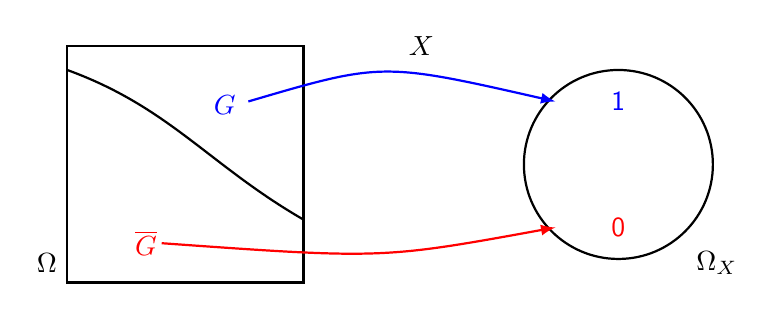
\begin{tikzpicture}[>=latex, font=\sffamily]
		
		% --- Conjunto Omega (quadrado à esquerda)
		\draw[thick] (0,0) rectangle (3,3) node[pos=0,above left] {$\Omega$};
		
		% Curva dividindo G e G-barra
		\draw[thick] (0,2.7) to[out=-20,in=150] (3,0.8);
		
		% Região G (em azul)
		\node[blue] at (2,2.25) {$G$};
		
		% Região G-barra (em vermelho)
		\node[red] at (1,0.5) {$\overline{G}$};
		
		% --- Conjunto OmegaY (círculo à direita)
		\draw[thick] (7,1.5) circle (1.2);
		
		\node at (8.25, 0.25) {$\Omega_X$};
		% Elementos 0 e 1 dentro do círculo
		\node[blue] at (7,2.3) {1};
		\node[red] at (7,0.7) {0};
		
		% --- Função Y (as setas)
		\node at (4.5,3) {$X$};
		
		\draw[->,blue,thick] (2.3,2.3) .. controls (4,2.8) .. (6.2,2.3);
		\draw[->,red,thick] (1.2,0.5) .. controls (4,0.3) .. (6.2,0.7);
		
	\end{tikzpicture}
\end{document}
